% Netanomics Slide Template in Beamer
%Jonathan H. Morgan
%19 February 2024

\documentclass[t, aspectratio=169]{beamer}

\usepackage{Netanomics_Beamer}

\title{Netanomics Template}
\subtitle{Standalone}
\author{Jonathan H. Morgan, Ph.D.}
\date{20 February 2024}

\begin{document}

% Apply the title page background just before the title page
\setTitlePageBackground
\begin{frame}[plain]
  \titlepage
\end{frame}

%Table of Contents
\setMainSlideBackground
\begin{frame}
    \frametitle{\shadowtext{Table of Contents}}
    \tableofcontents
\end{frame}

%Presentation Slides
\section{Basic Slides}

\begin{frame}
    \frametitle{Basic Text}
    {\fontfamily{ppl}\selectfont This is an example of the main text in Palatino Linotype.} The title above is set in Lucida Sans Unicode with a shadow effect.
\end{frame}

\begin{frame}
    \frametitle{Bullets}
    \begin{itemize}
        \item Create OMEN Release Checklist
        \item Create BEND Initial Changes Slides
    \end{itemize}
\end{frame}

\section{Special Environments}

\begin{frame}
    \frametitle{Special Environments}
    \begin{block}{Note}
        The validity of a global Social Network Analysis depends on the completeness of the analyzed network.
    \end{block}

    \begin{example}
        For more information \href{https://www.youtube.com/watch?v=rx7wwtmFlD8&list=PLHXZ9OQGMqxcWWkx2DMnQmj5os2X5ZR73&index=9}{see}
    \end{example}

    \begin{theorem}[Pythagoras]
        $a^2 + b^2 = c^2$
    \end{theorem}
\end{frame}

\begin{frame}
    \frametitle{Text and Graphics}
    \begin{columns}[T]
    \column{0.5\textwidth}
    \vspace{-1em} % Adjust the value as needed
    {\footnotesize % This command sets the font size for the content within the curly braces
    \begin{equation*}
        y_{ij} = \beta_0 + \sum_{k=1}^{n} \beta_{k} \cdot X_{ijk} + \epsilon_{ij}
    \end{equation*}
     \vspace{-0.9em} % Adjust the value as needed
    where:
    \begin{itemize}
        \setlength\itemsep{1em} % Optional: Adjusts the space between items
        \item[] \(y_{ij}\) represents the count of maneuvers,
        \item[] \(\beta_0\) is the intercept,
        \item[] \(\beta_k\) are the coefficients reflecting the impact of each account and maneuver,
        \item[] \(X_{ijk}\) denotes the presence (1) or absence (0) of maneuver \(i\) by account \(j\),
        \item[] \(\epsilon_{ij}\) is the error term, indicating the residuals.
    \end{itemize}
    }

    \column{0.5\textwidth}
    \begin{figure}
        \centering % This centers your figure
        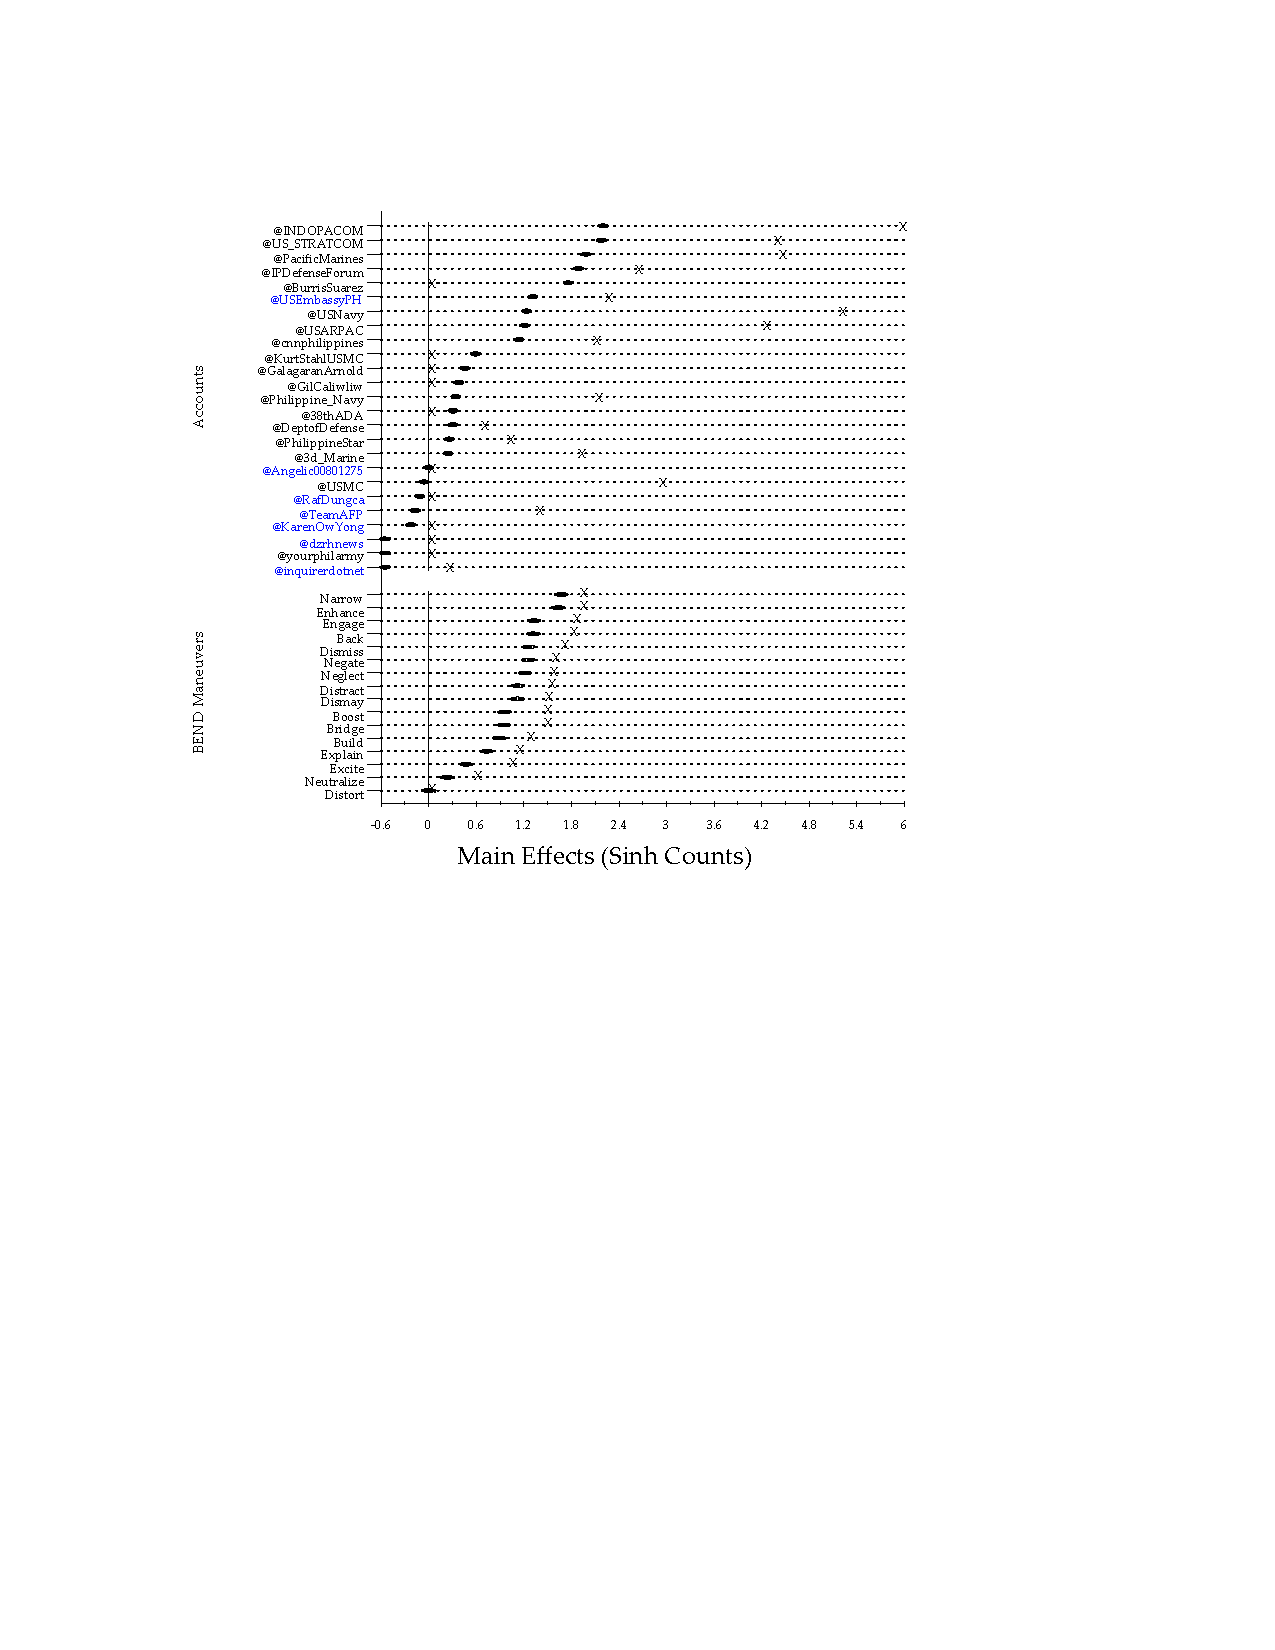
\includegraphics[width=0.9\linewidth, keepaspectratio]{Balikatan_2022_BEND_Media_Main_Effects.pdf}%
        \caption*{}
        \label{}
    \end{figure}
    \end{columns}
\end{frame}


\end{document}
